\documentclass[12pt,a4paper]{report}
\usepackage[utf8]{inputenc}
\usepackage{amsmath}
\usepackage{amsfonts}
\usepackage{amssymb}
\usepackage{amsthm}
\usepackage{hyperref}

\usepackage{multicol}
\usepackage{fancyhdr}
\usepackage[inline]{enumitem}
\usepackage{tikz}
\usepackage{tikz-cd}
\usetikzlibrary{calc}
\usetikzlibrary{shapes.geometric}
\usetikzlibrary{positioning}
\usepackage[margin=0.5in]{geometry}
\usepackage{xcolor}

\hypersetup{
    colorlinks=true,
    linkcolor=blue,
    filecolor=magenta,      
    urlcolor=cyan,
    pdftitle={Tensors},
    pdfpagemode=FullScreen,
    }

%\urlstyle{same}

\newcommand{\CLASSNAME}{Math 5050 -- Special Topics: Tensor Analysis}
\newcommand{\STUDENTNAME}{Paul Carmody}
\newcommand{\ASSIGNMENT}{Presentation \#1 }
\newcommand{\DUEDATE}{February 4, 2026}
\newcommand{\PROFESSOR}{Professor Berchenko-Kogan}
\newcommand{\SEMESTER}{Spring 2026}
\newcommand{\SCHEDULE}{TBD}
\newcommand{\ROOM}{Remote}

\newcommand{\MMN}{M_{m\times n}}
\newcommand{\FF}{\mathcal{F}}

\pagestyle{fancy}
\fancyhf{}
\chead{ \fancyplain{}{\CLASSNAME} }
%\chead{ \fancyplain{}{\STUDENTNAME} }
\rhead{\thepage}

\fancyfoot{} % clear all footer fields
\fancyfoot[LE,RO]{\thepage}
\fancyfoot[LO,CE]{-------\\\ASSIGNMENT}
%\fancyfoot[CO,RE]{To: Dean A. Smith}
\input{../MyMacros}

\newcommand{\RED}[1]{\textcolor{red}{#1}}
\newcommand{\BLUE}[1]{\textcolor{blue}{#1}}

\newcommand{\SUPP}{\operatorname{supp}}
\newcommand{\CLOSURE}{\operatorname{closure of}}
\newcommand{\BD}{\operatorname{bd}}
\newcommand{\HHN}{\mathcal{H}^n}
\newcommand{\COFF}[3]{\Gamma^{#1}_{{#2}{#3}}}
\newcommand{\VK}[1]{\textbf{#1}}
\newcommand{\VKR}{\VK{R}}
\newcommand{\VKZ}{\VK{Z}}

\begin{document}

\begin{center}
	\Large{\CLASSNAME -- \SEMESTER} \\
	\large{ w/\PROFESSOR}
\end{center}
\begin{center}
	\STUDENTNAME \\
	\ASSIGNMENT -- \DUEDATE\\
\end{center} 

\textbf{\large{Exercises}}
Chapter 2: 6, 7, 14
Chapter 3: 21, 22, 23
Chapter 4: 46, 48, 53
Chapter 5: 63

\begin{enumerate}[label=\textbf{2.\arabic*.}]
\setcounter{enumi}{5}
\item Demonstrate geometrically that the dot product is distributive.

First consider a simply expression $(\vec{A} +\vec{B})\cdot\vec{i}$\\
\begin{center}

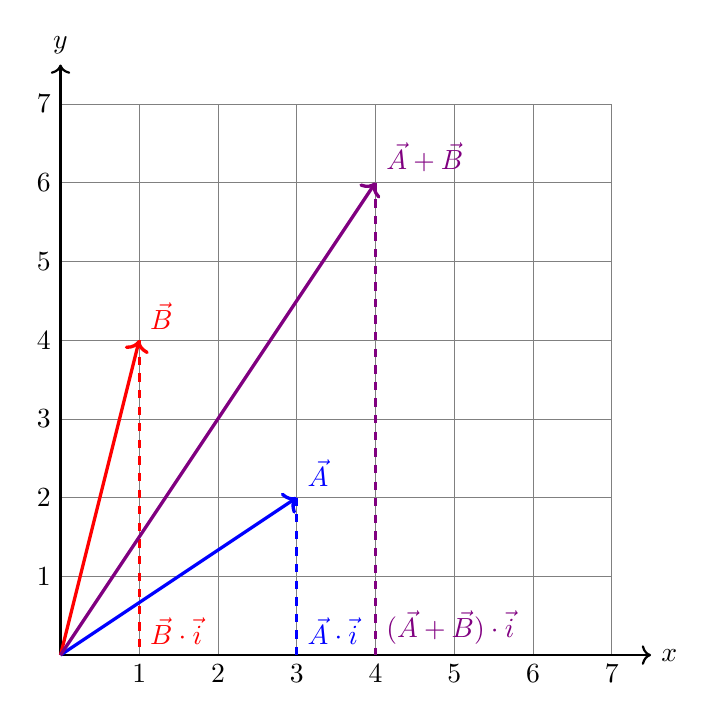
\begin{tikzpicture}
    % 1. Draw the grid with light gray, thin lines and 1cm step size
    \draw[step=1cm, gray, very thin] (0,0) grid (7,7);

    % 2. Draw the axes (optional, but helpful for context)
    \draw[->, thick] (0,0) -- (7.5,0) node[right] {$x$};
    \draw[->, thick] (0,0) -- (0,7.5) node[above] {$y$};

    % 3. Add coordinates for context (optional)
    \foreach \x in {1, 2, 3, 4, 5, 6, 7} {
        \node[below] at (\x, 0) {$\x$};
    }
    \foreach \y in {1, 2, 3, 4, 5, 6, 7} {
        \node[left] at (0, \y) {$\y$};
    }

    % 4. Draw a vector from the origin (0,0) to the point (3, 2)
    % The "->" option creates an arrow head
    \draw[->, very thick, blue] (0,0) -- (3,2) node[above right] {$\vec{A}$};

    % 4a. Draw a vector from the origin (0,0) to the point (3, 2)
    % The "->" option creates an arrow head
    \draw[dashed, very thick, blue] (3,2) -- (3,0) node[above right] {$\vec{A}\cdot\vec{i}$};
    
    % 5. Draw a vector from the origin (0,0) to the point (3, 2)
    % The "->" option creates an arrow head
    \draw[->, very thick, red] (0,0) -- (1,4) node[above right] {$\vec{B}$};
    
    % 5a. Draw a vector from the origin (0,0) to the point (3, 2)
    % The "->" option creates an arrow head
    \draw[dashed, very thick, red] (1,4) -- (1,0) node[above right] {$\vec{B}\cdot \vec{i}$};
    
    % 6. Draw a vector from the origin (0,0) to the point (3, 2)
    % The "->" option creates an arrow head
    \draw[->, very thick, violet] (0,0) -- (4,6) node[above right] {$\vec{A}+\vec{B}$};
    
    % 6. Draw a vector from the origin (0,0) to the point (3, 2)
    % The "->" option creates an arrow head
    \draw[dashed, very thick, violet] (4,6) -- (4,0) node[above right] {($\vec{A}+\vec{B})\cdot\vec{i}$};

\end{tikzpicture}
\end{center}
we can clearly see that $\vec{B}\cdot\vec{i} = 1$ and $\vec{A}\cdot\vec{i} = 3$ and $(\vec{A}+\vec{B})\cdot\vec{i} = 4$.\\

Now consider another simple expression $(\vec{A} +\vec{B})\cdot\vec{j}$\\
\begin{center}

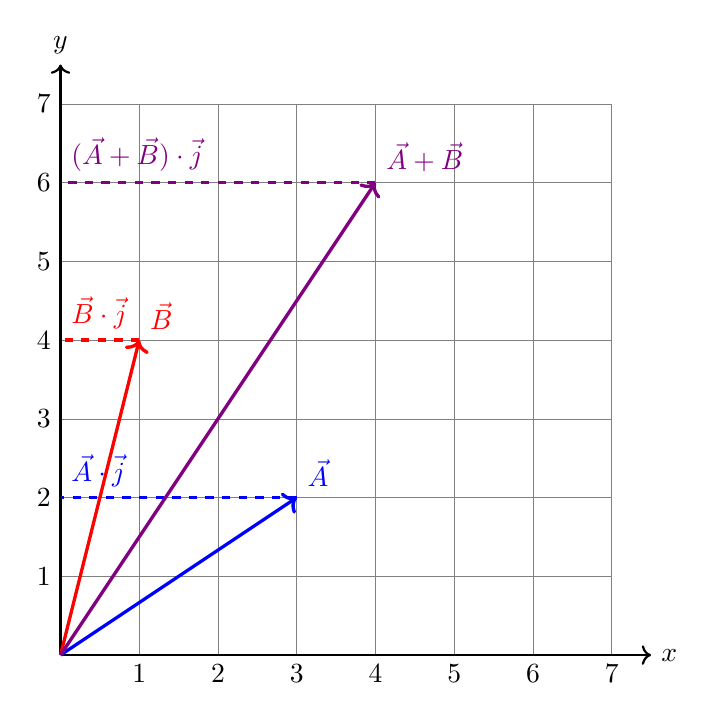
\begin{tikzpicture}
    % 1. Draw the grid with light gray, thin lines and 1cm step size
    \draw[step=1cm, gray, very thin] (0,0) grid (7,7);

    % 2. Draw the axes (optional, but helpful for context)
    \draw[->, thick] (0,0) -- (7.5,0) node[right] {$x$};
    \draw[->, thick] (0,0) -- (0,7.5) node[above] {$y$};

    % 3. Add coordinates for context (optional)
    \foreach \x in {1, 2, 3, 4, 5, 6, 7} {
        \node[below] at (\x, 0) {$\x$};
    }
    \foreach \y in {1, 2, 3, 4, 5, 6, 7} {
        \node[left] at (0, \y) {$\y$};
    }

    % 4. Draw a vector from the origin (0,0) to the point (3, 2)
    % The "->" option creates an arrow head
    \draw[->, very thick, blue] (0,0) -- (3,2) node[above right] {$\vec{A}$};

    % 4a. Draw a vector from the origin (0,0) to the point (3, 2)
    % The "->" option creates an arrow head
    \draw[dashed, very thick, blue] (3,2) -- (0,2) node[above right] {$\vec{A}\cdot\vec{j}$};
    
    % 5. Draw a vector from the origin (0,0) to the point (3, 2)
    % The "->" option creates an arrow head
    \draw[->, very thick, red] (0,0) -- (1,4) node[above right] {$\vec{B}$};
    
    % 5a. Draw a vector from the origin (0,0) to the point (3, 2)
    % The "->" option creates an arrow head
    \draw[dashed, very thick, red] (1,4) -- (0,4) node[above right] {$\vec{B}\cdot \vec{j}$};
    
    % 6. Draw a vector from the origin (0,0) to the point (3, 2)
    % The "->" option creates an arrow head
    \draw[->, very thick, violet] (0,0) -- (4,6) node[above right] {$\vec{A}+\vec{B}$};
    
    % 6. Draw a vector from the origin (0,0) to the point (3, 2)
    % The "->" option creates an arrow head
    \draw[dashed, very thick, violet] (4,6) -- (0,6) node[above right] {($\vec{A}+\vec{B})\cdot\vec{j}$};

\end{tikzpicture}
\end{center}
we can clearly see that $\vec{B}\cdot\vec{j} = 4$ and $\vec{A}\cdot\vec{j} = 2$ and $(\vec{A}+\vec{B})\cdot\vec{j} = 6$.\\

This allows for any inner product of the form $(\vec{a}+\vec{B})\cdot(\vec{i}+\vec{j})$.  For the general case of $\alpha \vec{i}+\beta\vec{j}$ it is easy to see that $\alpha$ and $\beta$ also distribute due to the Distribution Law of Algebra.

%section 2.6
\item Evalute $d F/dl$ for $F(P) = $ ``Distance from $P$ to point $A$" in a direction perpendicular to $AP$.

\BLUE{$F(P) = d(P, A)$.  Let $l$ be perpendicular to $AP$ at $P$.  For any $p \in l,\, F(P+p) \to F(P)$ as $p \to P$.  That is, $\partial F/\partial l = F(P)$.  Geometrically, consider a circle centered at $A$ and going through $P$.  The line $l \perp AP$ is a tangent line, thus $\partial F/\partial l$ is simply following along a circle of the same radius as $d(A,P)$.
}


\setcounter{enumi}{13}
\item Give the geometric intuition behind equation (2.11). In other words, explain geometrically, why knowing the gradient is sufficient to determine the directional derivatives in all possible directions.

\BLUE{\begin{align*}
	\frac{dF}{dl} &= \nabla F\cdot \VK{L}
\end{align*}where $\VK{L}$ is the unit vector in the direction of $l$.  Interpreted directly, we can see that this means that change in $F$ along the $l$ is the projection of the gradient of $F$, $\nabla F$, onto the line $l$, i.e., $\nabla F \cdot \VK{L}$ in the direction of $\VK{L}$. 
\begin{itemize}
\item If $\nabla F$ is not parallel to $\VK{L}$ we have two vectors which combined by the cross product $\nabla F \times \VK{L}$ form three linearly independent vectors, hence, a basis.
\item If $\nabla F$ is parallel to $\VK{L}$ then $\nabla F$ can be considered the normal vector to a plane.  This plane can be described by vectors perpendicular to each other and, by definition, perpendicular to $\nabla F$, thus forming a set of basis.
\end{itemize}
}

\end{enumerate}
\HLINE

\begin{enumerate}[label=\textbf{3.\arabic*}]
\setcounter{enumi}{20}
\item Given a polar coordinate system, introduce Cartesian coordinates that originate at the same pole and for which the $x$-axis coincides withthe polar axis.  Show that the Cartesian coordinates $(x,y)$ are related to the polar coordinates $(r,\theta)$ by the following identities:
\begin{align*}
	x(r,\theta) = r\cos \theta \\
	y(r,\theta) = r\sin \theta
\end{align*} 
\begin{center}

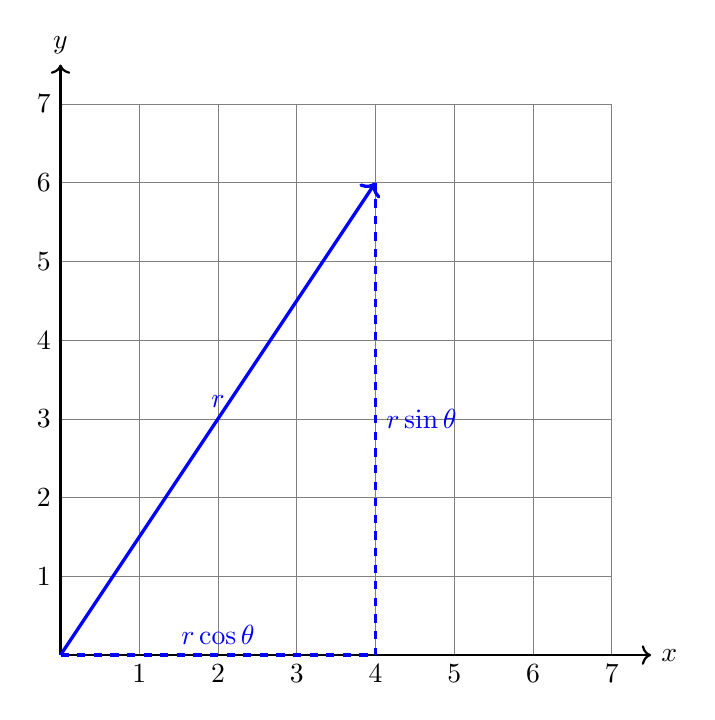
\begin{tikzpicture}
    % 1. Draw the grid with light gray, thin lines and 1cm step size
    \draw[step=1cm, gray, very thin] (0,0) grid (7,7);

    % 2. Draw the axes (optional, but helpful for context)
    \draw[->, thick] (0,0) -- (7.5,0) node[right] {$x$};
    \draw[->, thick] (0,0) -- (0,7.5) node[above] {$y$};

    % 3. Add coordinates for context (optional)
    \foreach \x in {1, 2, 3, 4, 5, 6, 7} {
        \node[below] at (\x, 0) {$\x$};
    }
    \foreach \y in {1, 2, 3, 4, 5, 6, 7} {
        \node[left] at (0, \y) {$\y$};
    }

    % 4. Draw a vector from the origin (0,0) to the point (3, 2)
    % The "->" option creates an arrow head
    \draw[->, very thick, blue] (0,0) -- (4,6) node[midway, above ] {$r$};

    % 4. Draw a vector from the origin (0,0) to the point (3, 2)
    % The "->" option creates an arrow head
    \draw[dashed, very thick, blue] (4,6) -- (4,0) node[midway, right ] {$r\sin \theta$};    

    % 4. Draw a vector from the origin (0,0) to the point (3, 2)
    % The "->" option creates an arrow head
    \draw[dashed, very thick, blue] (0,0) -- (4,0) node[midway, above ] {$r\cos \theta$};    
\end{tikzpicture}
\end{center}


\item Show that the inverse relationship is
\begin{align*}
	r(x,y) &= \sqrt{x^2+y^2} \\
	\theta(x,y) &= \arctan \frac{y}{x}
\end{align*}

\BLUE{\begin{align*}
	x(r,\theta)^2 + y(r, \theta)^2 &= r^2\cos^2\theta+r^2\sin^\theta = r^2 \implies r(x,y) = \sqrt{x^2+y^2}  \\
	\tan \theta &= \frac{\sin\theta}{\cos\theta} = \frac{r\sin\theta}{r\cos\theta} \frac{y}{x} \implies \theta = \arctan\frac{y}{x}
\end{align*}
}

\item Align a Cartesian coordinate system $x,y,z$ with a given cylindrical coordinate system in a natural way.  Show that $x,y,z$ and $r, \theta, z$ (we hop it is OK to reuse the letter $z$) are related as follows
\begin{align*}
	x(r,\theta,z) &= r\cos \theta\\
	y(r,\theta,z) &- \arctan\frac{y}{x} \\
	z(x,y,z) &= z
\end{align*}

\BLUE{Give cylindrical coordinates $(r, \theta, z)$, we can make Cartesian coordinates $(x,y,z)$ where the $x$-axis cooresponds to $\theta = 0$ and the $z$-axis is the same in both.  Consequently, as in 21 above, any point $p=(r, \theta)$  will have projections onto the $x$ and $y$ axes as 
\begin{align*}
	x(r, \theta, z) &= r\cos \theta \\
	y(r, \theta, z) &= r\sin \theta \\
	z(r, \theta, z) &= z.
\end{align*}Alternatively, we can envision a vector $\VK{P} = (r, \theta)$ projected onto the $x$-axis with the unit vector $\hat{i}$.  $\VK{P} \cdot \hat{i} = |\VK{P}|\,|\hat{i}|\cos\theta = r\cos\theta$. And similarly for the unit vector of the $y$-axis, $\hat{j}$.
}

\end{enumerate}
\HLINE

\begin{enumerate}[label=\textbf{4.\arabic*}]

\setcounter{enumi}{45}
	\item \textbf{Pg 47}  By differentiation
	\begin{align*}
		Z^{i'}(Z(Z'))=Z'
	\end{align*}show that 
	\begin{align*}
		J_i^{i'}J_{j'}^i= \delta^{i'}_{j'}
	\end{align*}
	
	\BLUE{Where
	\begin{align*}
		Z^i(Z'(Z)) \equiv Z^i
	\end{align*}or by identity
	\begin{align*}
		Z^{i'}(Z(Z')) \equiv Z^{i'}
	\end{align*}and
	\begin{align*}
		J_{i'}^i &= \PART{Z^i(Z)}{Z^{i'}} & \quad
		J_i^{i'} &= \PART{Z^{i'}(Z)}{Z^i} \\
			&= \PART{Z^i}{Z}\PART{Z}{Z^{i'}} & \quad &= \PART{Z^{i'}}{Z}\PART{Z}{Z^i}
	\end{align*}which follows that
	\begin{align*}
		J_i^{i'}J_{j'}^i &= \PART{Z^{i'}(Z)}{Z^i}\PAREN{\PART{Z^i(Z)}{Z^{i'}}} \\
		&= \PART{Z^{i'}}{Z}\PART{Z}{Z^i}\PAREN{\PART{Z^i}{Z}\PART{Z}{Z^{j'}}} \\
		&= \PART{Z^{i'}}{Z^{j'}} \\
		&= \delta_{j'}^{i'}
	\end{align*}
	}

\setcounter{enumi}{47}
	
	\item \textbf{Pg 47} Introduce the symbols $J_{i'j'}^i$ and $J_{ij}^{i'}$ for the second order partial derivatives
	\begin{align*}
		J_{i'j'}^i &= \frac{\partial^2 Z^i(Z')}{\partial Z^{i'}\partial Z^{j'}}\\
		J_{ij}^{i'} &= \frac{\partial^2 Z^{i'}(Z)}{\partial Z^{i}\partial Z^{j}}.
	\end{align*}Show that
	\begin{align*}
		J_{i'j'}^iJ_j^{i'}J_k^{j'}+J_{i'}^iJ_{jk}^{i'}=0.
\end{align*}	 How many identities does this tensor relationship represent?
	
	\BLUE{Let's begin with 
	\begin{align*}
		J_i^{i'}J_{j'}^i &=\delta_{j'}^{i'} \\
		\frac{\partial}{\partial Z^k}\delta_{j'}^{i'} &=\frac{\partial}{\partial Z^k}\PAREN{J_i^{i'}J_{j'}^i} \\
		0 &= \frac{\partial}{\partial Z^k}\PAREN{J_i^{i'}}J_{j'}^i + J_i^{i'}\frac{\partial}{\partial Z^k}\PAREN{J_{j'}^i}\\
		&= J_{ik}^{i'}J_{j'}^i+J_i^{i'}J_{kj'}^i
	\end{align*}
	}

\setcounter{enumi}{52}
	
	\newcommand{\JJJ}[2]{J^{#1}_{#2}}
	\newcommand{\JJJJ}[2]{\frac{\partial Z^{#1}(Z)}{\partial Z^{#2}}}
	\item \textbf{Pg 47} Consider the three changes of variable: $Z^i$, $Z^{i'}$, $Z^{i''}$ and back to $Z^i$.  Show that
	\begin{align*}
		\JJJ{i}{i'}\JJJ{i'}{i''}\JJJ{i''}{j}	&= \delta^i_j
	\end{align*}
	
	\BLUE{\begin{align*}
		\JJJ{i}{i'}\JJJ{i'}{i''}\JJJ{i''}{j}	&= \JJJJ{i}{i'}\JJJJ{i'}{i''}\JJJJ{i''}{j} \\
		&= \JJJJ{i}{}\PART{Z}{Z^{i'}}\JJJJ{i'}{}\PART{Z}{Z^{i''}}\JJJJ{i''}{}\PART{Z}{Z^j} \\
		&= \PART{Z^i(Z)}{Z^{i'}}\PART{Z^{i'}(Z)}{Z^{i''}}\PART{Z^{i''}(Z)}{Z^{j}} \\
		&= \PART{Z^i(Z)}{Z^{j}} \\
		&=  \delta^i_j
	\end{align*}
	}

\end{enumerate}

\HLINE
\begin{enumerate}[label=\textbf{5.\arabic*}]
\setcounter{enumi}{62}


\item Show that the length $|\VK{V}|$ of a vector $\VK{V}$ is given by \begin{align*}
	|\VK{V}| &= \sqrt{Z_{ij}V^iV^j}.
\end{align*}

\BLUE{\begin{align*}
	\VK{V} &= (V^i) \\
	|\VK{V}| &= \sqrt{\VK{V}\cdot\VK{V}} \\
	&= \sqrt{V^i\VK{Z}_i\cdot V^j\VK{Z}_j}\\
	&= \sqrt{V^iV^j(\VK{Z}_i\cdot \VK{Z}_j)}\\
	&= \sqrt{V^iV^j Z_{ij}}
\end{align*}
}

\end{enumerate}
\end{document}